\chapter{Analysis and evaluation}\label{cap:analysis}

This chapter documents the implementation of the following techniques used to improve the chess engine:

\begin{itemize}[itemsep=1pt]
    \item Transposition tables with zobrist hashing.
    \item Move generator with magic bitboards and PEXT instructions.
    \item Evaluation with king safety and piece mobility parameters.
    \item Multithread search.
    \item Search with Late move Reductions.
\end{itemize}


\newpage

\noindent Achieving this level of efficiency and quality requires a well-structured development process. For this reason, we adopted a systematic methodology to guide the implementation and continuous improvement of our engine.

\section{Methodology}

Once the basic foundations are established with an initial version of the essential components or modules (which will be described later), our workflow follows an iterative process: first, we search for existing information on each topic, analyze it, implement a solution, and then profile the implementation to identify bottlenecks. After locating performance issues, we optimize the relevant parts, and finally, compare the new version with the previous one to assess improvements.

\vspace{1em}

\noindent Then, at a given moment, we can decide to take action and try to determine the strength of the engine with the last functional version.

\subsection*{Profiler}

First, in order to analyze the performance of our chess engine and identify potential bottlenecks, we used the \texttt{perf} tool available on Linux systems. \texttt{perf} provides robust profiling capabilities by recording CPU events, sampling function execution, and collecting stack traces.

\vspace{1em}

\noindent Our profiling goal is to identify which parts of the code consume the most execution time. We run the engine under \texttt{perf} using the following commands:

\begin{lstlisting}[language=bash, caption={Profiling AlphaDeepChess with perf}, frame=single, breaklines=true]
# Record performance data with function stack traces
sudo perf record -g ./build/release/AlphaDeepChess

# Display interactive report
sudo perf report -g --no-children
\end{lstlisting}

\noindent After recording, \texttt{perf report} opens an interactive terminal interface where functions are sorted by CPU overhead. This allows us to prioritize which functions to optimize.

\noindent The most common way to measure the strength of a chess engine is by playing games against other engines and analyzing the results. To quantify this strength, the Elo rating system is used. Elo is a statistical rating system originally developed for chess, which assigns a numerical value to each player (or engine) based on their game results against opponents of known strength. When an engine wins games against higher-rated opponents, its Elo increases; if it loses, its Elo decreases. This allows for an objective comparison of playing strength between different engines.

\vspace{1em}

\noindent But which engine should we use as a reference for comparison? One approach is to consult the Computer Chess Rating Lists, which rank chess engines based on their performance in various tournaments and matches. We have chosen to compare different versions of our engine with \textit{Stockfish}, currently ranked as the number one engine on the list. In addition, we have also competed against other engines online to further evaluate our engine's performance in diverse environments.

\vspace{1em}

\noindent We created a benchmark to measure the effectiveness of each technique by playing matches with 100 games versus a baseline engine implementation, and we analyze the results of these games at the end of the process to assess the impact of each improvement.


All of these improvements have been compared with each other using \textit{CuteChess}, and the best version was also evaluated against \textit{Stockfish}. These comparisons were conducted on machines provided by GitHub Actions.

\subsection*{Cutechess}

\noindent After considering different options, \textit{Cutechess} proved to be the best fit for our needs.

\vspace{1em}

\noindent \textit{Cutechess}~\cite{CuteChess} is an open-source tool designed to perform automated games between chess engines. It is widely used in the chess programming community to test and compare engines, evaluate their performance, and analyze games.

\vspace{1em}

\noindent It provides both command-line interface (CLI) and a graphic user interface (GUI), with cross-platform compatibility for Windows, macOS, and Linux. For our purposes, we utilized the CLI version to automate the tests with Python scripts and commands, integrating it into a CI/CD workflow.

\vspace{1em}

\noindent Mainly, this tool is responsible for sending commands to both selected engines. For example, when both Stockfish and our engine implement UCI, \textit{Cutechess} knows in advance the commands to send, as well as parameters such as the search time and depth for each engine, the number of games to play, the time control, or even specific openings to use. Providing specific openings introduces randomization between games, which is beneficial for later evaluation.

\vspace{1em}

\noindent Then, it checks the active status of each engine and manages the start of the games by setting up the board on both engines with the \texttt{position} command. Afterwards, it sends the \texttt{go} command and stops the search with \texttt{stop} when the search time or depth is reached, extracting the best move provided by the engine whose turn it is. This move is then passed to the other engine, alternating turns so that both engines play against each other automatically.~\cref{lst:cutechess-example} we show a \textit{Cutechess} log file, we directly configured the starting positions from a list of FENs in the \texttt{positions.fen} file:

\begin{lstlisting}[basicstyle=\ttfamily\scriptsize, breaklines=true, frame=single, caption={Example of \textit{Cutechess}}, label={lst:cutechess-example}]
Running test (8) with the following configuration:
Games: 1, Search Time: 5, Depth: 5
PGN File: results.pgn, EPD File: results.epd, Log File: results.log
Engines: ['AlphaDeepChess', 'Stockfish']
Options: {'Stockfish': {'UCI_LimitStrength': 'true', 'UCI_Elo': '2000'}}
Book: 
Positions: positions.fen
...
 <Stockfish(1): uciok
 >Stockfish(1): setoption name UCI_Elo value 2000
 >Stockfish(1): setoption name UCI_LimitStrength value true
 >Stockfish(1): isready
 <Stockfish(1): readyok
Started game 1 of 1 (AlphaDeepChess vs Stockfish)
 >AlphaDeepChess(0): ucinewgame
 >AlphaDeepChess(0): position fen rnbqkb1r/1p2pppp/p2p1n2/8/3NP3/2N5/PPP2PPP/R1BQKB1R w KQkq - 0 6
 >Stockfish(1): ucinewgame
 >Stockfish(1): setoption name Ponder value false
 >Stockfish(1): position fen rnbqkb1r/1p2pppp/p2p1n2/8/3NP3/2N5/PPP2PPP/R1BQKB1R w KQkq - 0 6
 >AlphaDeepChess(0): isready
 <AlphaDeepChess(0): readyok
 >AlphaDeepChess(0): go movetime 5000 depth 5
 <AlphaDeepChess(0): info depth 1 score cp 130 bestMove c1e3
 <AlphaDeepChess(0): info depth 2 score cp 85 bestMove c1e3
 <AlphaDeepChess(0): info depth 3 score cp 80 bestMove c1e3
 <AlphaDeepChess(0): info depth 4 score cp 62 bestMove c1g5
 <AlphaDeepChess(0): info depth 5 score cp 79 bestMove c1g5
 <AlphaDeepChess(0): bestmove c1g5
 >Stockfish(1): position fen rnbqkb1r/1p2pppp/p2p1n2/8/3NP3/2N5/PPP2PPP/R1BQKB1R w KQkq - 0 6 moves c1g5
 >Stockfish(1): isready
 <Stockfish(1): readyok
 >Stockfish(1): go movetime 5000 depth 5
 <Stockfish(1): info depth 1 seldepth 6 multipv 1 score cp -52 ...
 <Stockfish(1): info depth 2 seldepth 3 multipv 1 score cp -45 ...
 <Stockfish(1): info depth 3 seldepth 3 multipv 1 score cp -39 ...
 <Stockfish(1): info depth 4 seldepth 3 multipv 1 score cp -39 ...
 <Stockfish(1): info depth 5 seldepth 3 multipv 1 score cp -27 ...
 <Stockfish(1): bestmove e7e6
 >AlphaDeepChess(0): position fen rnbqkb1r/1p2pppp/p2p1n2/8/3NP3/2N5/PPP2PPP/R1BQKB1R w KQkq - 0 6 moves c1g5 e7e6
\end{lstlisting}

\noindent In~\cref{lst:cutechess-example}, in addition to setting the number of games to $1$, the search time to $5$ seconds, and the search depth to $5$, we provided a list of starting positions, from which one is chosen at random. Each line starting with \texttt{position fen \ldots} establishes the FEN position and continues by adding the moves played.

\vspace{1em}

\noindent Note that both engines stop searching when depth of $5$ is reached and are verified to be ready after \texttt{isready} command.

\vspace{1em}

\noindent Depending on the number of games, search time, and time control, these tournaments between engines can take a long time to process. For this reason, we decided to use GitHub Actions and workflows to separate our development environment from the execution of performance and strength tests. This is explained later in~\cref{cap:analysisOfImprovements}.

\vspace{1em}

\noindent Although UCI implements the \texttt{diagram} command that draws the current position through standard output, making moves and showing the evaluation is somewhat a time-consuming task when debugging and testing while programming. We resorted to using an interface to help us do this job and a really fast solution was to use Python to make a GUI. In this case, one of the most used UI libraries was \textit{CustomTkinter} and it was used to build a friendly interface from scratch for bridging between executable and command sending. This tool can be used after compiling the engine and executing \texttt{AlphaDeepChessGUI.py} with Python.

\begin{figure}
    \centering
    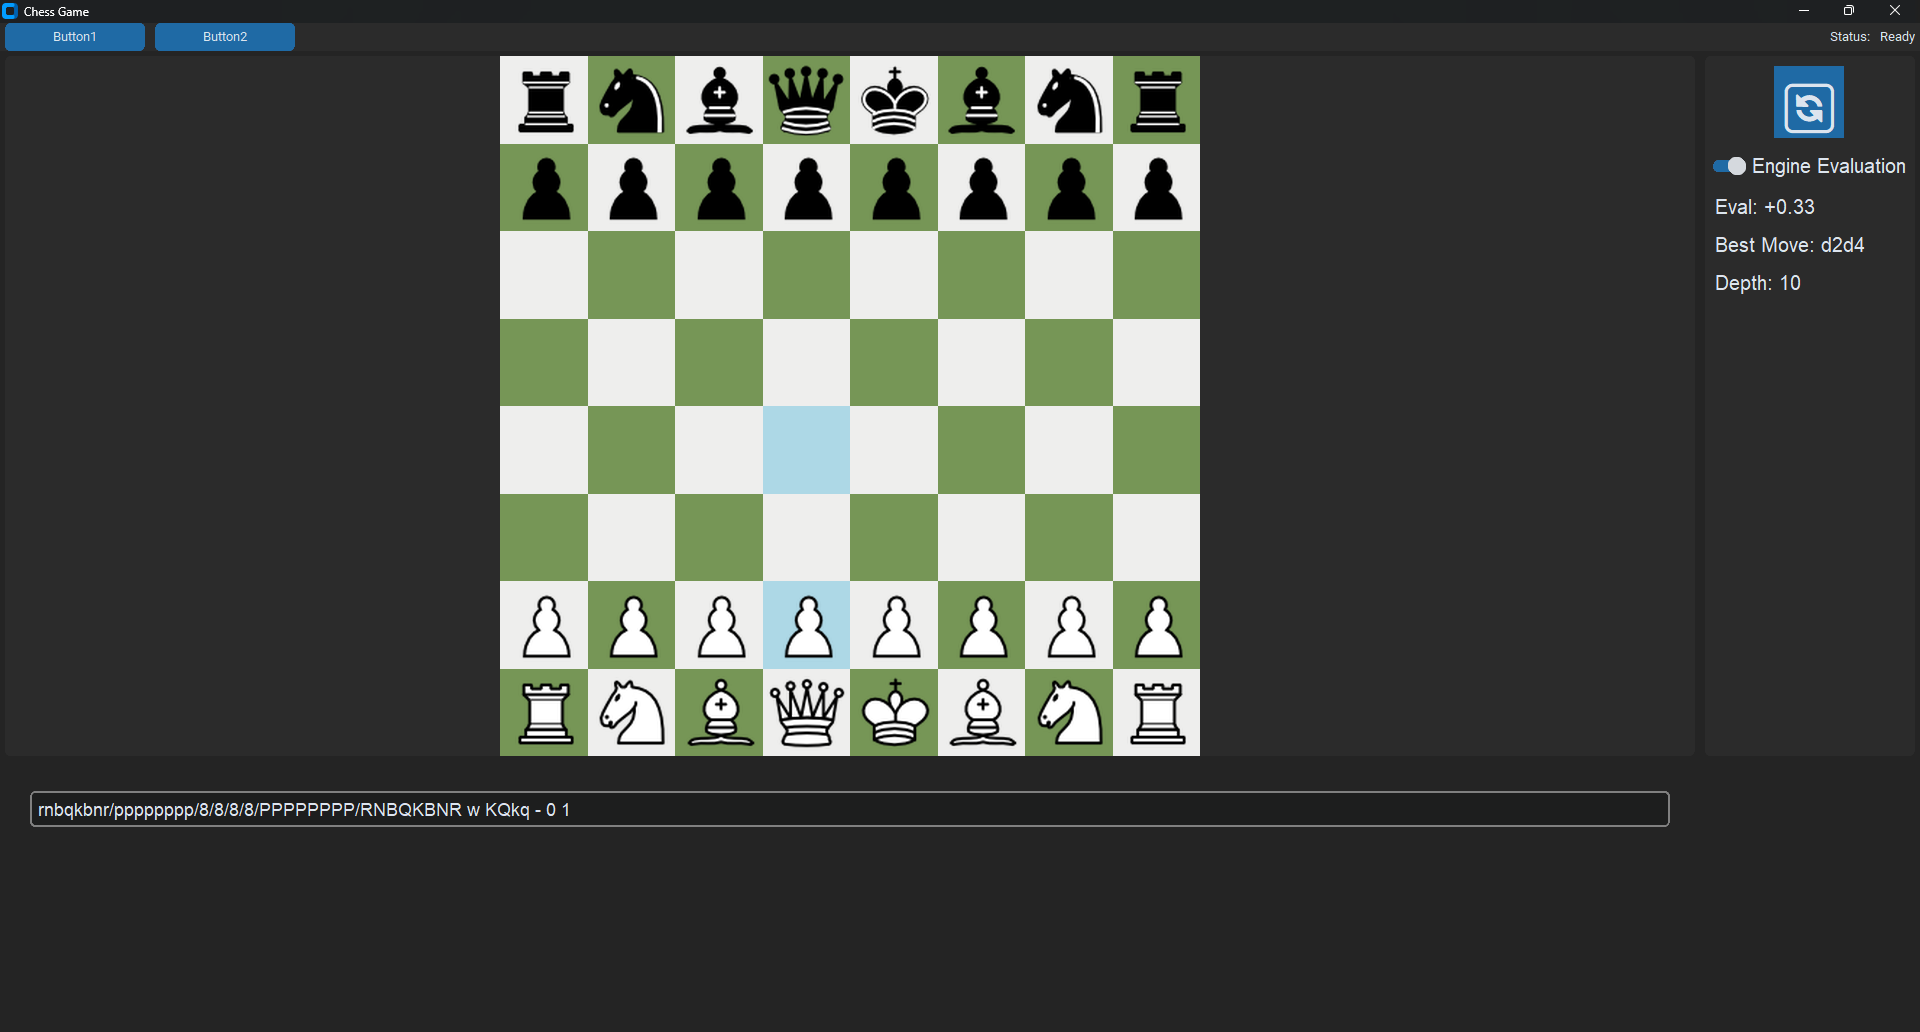
\includegraphics[width=1.0\textwidth]{Imagenes/gui.png}
    \caption{AlphaDeepChess GUI}\label{fig:gui}
\end{figure}

\noindent In~\cref{fig:gui}, the engine evaluation is enabled and displays the current evaluation value, the best move found, and the calculated search depth. In this way, we also ensure a more user-friendly experience.

\vspace{1em}

\section{Github actions and workflows}

GitHub Actions is a CI/CD tool integrated into GitHub that allows developers to automate tasks such as building, testing, and deploying code. Workflows are defined in YAML files and specify the tasks to be executed, the jobs or events that trigger them, and the environment in which they run.

\vspace{1em}

\noindent In this project, since it is public in a GitHub repository, we used GitHub Actions to automate the testing and evaluation of the chess engine with \textit{Stockfish} and \textit{CuteChess}. A workflow was configured (located at \texttt{.github\textbackslash{}workflows\textbackslash{}manual-workflow.yml}) to compile the engine and run automated games using \textit{CuteChess} between different versions of the engine or against \textit{Stockfish}.

\vspace{1em}

\noindent At the end of each section, we provide the results of a 100-game match between the improved engine and a baseline version. The baseline includes only the core techniques discussed in the previous chapter on engine architecture. The purpose of these matches is to measure the improvement in playing strength introduced by each new implementation.

\vspace{1em}

\noindent All matches are conducted using the tournament manager \textit{CuteChess}~\cite{CuteChess} with the following configuration:

\begin{itemize}[itemsep=1pt]
\item 100 games per match.
\item 50 unique random starting positions, each played twice with alternating colors.
\item 4 seconds of thinking time per move.
\item A 150-move limit per game, after which the game is declared a draw.
\end{itemize}

\noindent The matches were executed on virtual machines provided by GitHub Actions, using the \texttt{ubuntu-latest} runner. At the time of testing, this environment provided 4 CPUs, 16~GB of RAM, a 14~GB SSD, and a 64-bit architecture.

\section{Transposition table}\label{sec:tt}

\subsection*{Analysis}

\noindent To evaluate the impact of introducing the transposition table, we conducted the 100-game tournament against the baseline version of the engine. The~\cref{tab:tt_vs_basic} details the implementation used for each bot.

\vspace{1em}

\begin{table}
    \centering
    \begin{tabular}{|p{4cm}|p{4cm}|p{4cm}|}
    \hline
    \textit{Component}         & \textit{Transposition Table Bot}  & \textit{Basic Bot}     \\ \hline
    Search                     & Alpha-beta With Transposition Table          & Basic Alpha-beta           \\ \hline
    Evaluation Function        & Materialistic                      & Materialistic       \\ \hline
    Move Generator             & Basic implementation              & Basic implementation   \\ \hline
    Move Ordering              & MVV-LVA                           & MVV-LVA                \\ \hline
    \end{tabular}
    \caption{Match configuration: Transposition Table Bot vs Basic Bot}\label{tab:tt_vs_basic}
\end{table}

\noindent As illustrated in following result bar, we see a substantial improvement by adding the transposition table with 46 wins versus 32 losses. The remaining 22 games ended in a draw.

\begin{center}
\ResultBar{15cm}{0.5cm}{46}{22}{32}
\medskip
\end{center}

\section{Move generator with magic bitboards and pext instructions}

\subsection*{Analysis}

\noindent To evaluate the impact of introducing the move generator accelerated with PEXT instructions, we conducted the 100-game tournament against the baseline version of the engine. The~\cref{tab:pext_vs_basic} details the implementation used for each bot.

\vspace{1em}

\begin{table}
    \centering
    \begin{tabular}{|p{4cm}|p{4cm}|p{4cm}|}
    \hline
    \textit{Component}         & \textit{PEXT instructions Bot}  & \textit{Basic Bot}     \\ \hline
    Search                     & Alpha-beta With Transposition Table          & Basic Alpha-beta           \\ \hline
    Evaluation Function        & Materialistic                      & Materialistic       \\ \hline
    Move Generator             & PEXT implementation              & Basic implementation   \\ \hline
    Move Ordering              & MVV-LVA                           & MVV-LVA                \\ \hline
    \end{tabular}
    \caption{Match configuration: PEXT instructions Bot vs Basic Bot}\label{tab:pext_vs_basic}
\end{table}

\noindent As illustrated in the following result bar, we achieved a significant performance improvement by adding the PEXT instructions with 46 wins versus 22 losses. The remaining 14 games ended in a draw.

\begin{center}
\ResultBar{15cm}{0.5cm}{64}{14}{22}
\medskip
\end{center}

\section{Evaluation with king safety and piece mobility}

\subsection*{Analysis}

To evaluate the impact of introducing the new parameters in the evaluation, we conducted the 100-game tournament against the baseline version of the engine. The~\cref{tab:safety_mobility_vs_basic} details the implementation used for each bot.

\vspace{1em}

\begin{table}
    \centering
    \begin{tabular}{|p{4cm}|p{4cm}|p{4cm}|}
    \hline
    \textit{Component}         & \textit{PEXT instructions Bot}  & \textit{Basic Bot}     \\ \hline
    Search                     & Alpha-beta With Transposition Table          & Basic Alpha-beta           \\ \hline
    Evaluation Function        & Safety and Mobility                      & Materialistic      \\ \hline
    Move Generator             & PEXT implementation              & Basic implementation   \\ \hline
    Move Ordering              & MVV-LVA                           & MVV-LVA                \\ \hline
    \end{tabular}
    \caption{Match configuration: King Safety and Piece mobility eval Bot vs Basic Bot}\label{tab:safety_mobility_vs_basic}
\end{table}

\noindent As illustrated in the following result bar, the results are slightly worse compared to the match using the material-only evaluation shown in the following result bar, with 62 wins and 30 losses. This decline may be attributed to the additional computational overhead introduced by evaluating the new parameters. Moreover, while concepts such as king safety and piece mobility are intuitively valuable to human players, the engine may struggle to consistently associate them with actual positional strength.

\begin{center}
\ResultBar{15cm}{0.5cm}{62}{8}{30}
\medskip
\end{center}

\section{Multithreaded search}

\subsection*{Analysis}

To evaluate the improvement in the new evaluation, we conducted the same 100 game match vs the basic bot version. 

\begin{center}
\ResultBar{15cm}{0.5cm}{32}{5}{63}
\medskip
\end{center}

\noindent The results are slightly worse compared to the match using the material-only evaluation, with 8 more losses than before. This may be due to the increased computational cost of evaluating these additional parameters. Furthermore, although these are abstract concepts commonly used by humans to assess positions, the engine may struggle to find a clear correlation between them and actual positional strength.

\section{Late move reductions}

\subsection*{Analysis}

To evaluate the improvement in the new evaluation, we conducted the same 100 game match vs the basic bot version.

\begin{center}
 \ResultBar{15cm}{0.5cm}{48}{15}{37}
\medskip
\end{center}

\noindent The results are worse, with 15 more losses than the version without this aggresive pruning. This could be because our move ordering is not that strong, and the best move in the position sometimes is in the last positions.

\newpage

\section{Evaluation versus stockfish}

\begin{center}
 \ResultBar{15cm}{0.5cm}{0}{0}{100}
\medskip
\end{center}

\noindent AlphaDeepChess lost all games against Stockfish. This outcome was expected, as Stockfish has an estimated Elo rating of around 3644~\cite{StockfishElo}, making it orders of magnitude stronger than the best human players. In contrast, as we will show in the next section, AlphaDeepChess plays at a level comparable to a strong human player.

\section{Engine final evaluation}

\noindent Figure~\cref{fig:eloDistribution} shows the Elo rating distribution of players on Lichess, where the median rating is approximately 1500.

\vspace{1em}

\noindent AlphaDeepChess has achieved a rating of 1900 on Lichess~\cite{AlphaDeepChessElo}, placing it well above the median and within the top percentiles of the player base. For comparison, the highest-rated human player on the platform has reached 3000 Elo in 2025~\cite{LichessBestPlayer}.

\begin{figure}
    \centering
    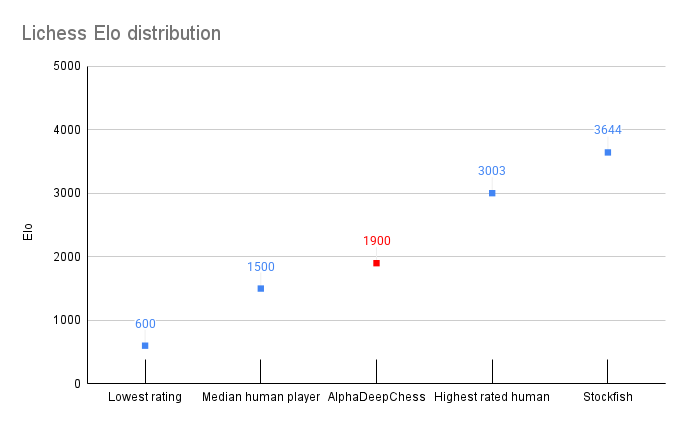
\includegraphics[width=0.95\linewidth]{Imagenes/eloDistribution.png}
    \caption{Lichess Elo distribution as of May 2025~\cite{LichessEloDistribution}.}
    \label{fig:eloDistribution}
\end{figure}